\chapter{Implementation}
This chapter aims to present the reader with explanation of the key implementation aspects. These include major challenges, problems that have been encountered and decisions that have been taken during the course of this project. I have tried to avoid going into too much technical details except where this is essential and provides the reader with better insight and understanding of the material.

The system I have developed as a prototype which to satisfy our aims consists of two sub systems. These are the disruption engine which address the first aim of detecting disruptions in the bus network, and a web front end application which to visualise the calculated disruptions. Below I have presented the major implementation decisions and challenges that were faced during the development of this system. We begin with first describing the data that has been provided by TFL for this project. Afterwards we go into discussion of the implementation of the disruption engine which captures the core functionality and business logic of the system. Then implementation of the visualisation part is discussed which can be viewed as an extension of the disruption engine.

\section{iBus AVL Data}
%Include a sample of the data and explanation of all fields
%Explain what the schedule deviation value means
%Include discussion on how the network is represented and the source of the file - TFL open data
%iBus system generate very short telegram messages with the bus location \cite{Hounsell201276}. This information is then processed on a server and more information is calculated and derived.
%The data that has been provided by Technical Service Group (TSG) at TFL for this project consists of preprocessed iBus feeds. This feeds currently are being generated every 5 minutes. Each file consists of the following fields:
%The information we are interested is the deviation from the schedule. This is calculated by knowing the expected arrival time of the bus at a stop from the schedule and is compared to the observed time. This value is calculated the same way for both low and high frequency buses(Low frequency buses are supposed to run according to a fixed schedule (e.g. a bus should arrive at stop at predefined time) and usually routes which have less than 5 buses an hour. High frequency bus routes should maintain headways - this meaning a bus should be arriving at stop at predefined intervals (e.g. each 2 minutes)). More about the supplied data for this project would be covered in the requirements section.
%Key property of time series data is stationarity. This means that the behaviour of the time series data does not change over time. In our case the data generally speaking the time series data is not stationary. However if we consider short window size it might be possible to treat the data as close to stationary.
The data that is used for this project is provided by the Technical Service Group (TSG) at TFL. This data consists of comma separated value (CSV) files. There is an individual file for every different bus operator which contains the data for all buses currently operated by this company. Initially every bus in the network would transmit its unique identification number and GPS coordinates approximately every 30 seconds \cite{Hounsell201276}. This information is then preprocessed by a central server. This results in more information being derived as the central server has knowledge of the whole network and the bus schedules and headways. This results in the CSV feed files that have been provided to us for this project. An example of the content of the raw feed file and a formatted version is presented in figure~\ref{fig:rawDataSample} and ~\ref{fig:formattedDataSample} respectively . Below I have provided a detailed explanation of each field in these files \cite{infoBusesInservice}.
\begin{itemize}
	\item \textbf{Vehicle Id} - this is a unique id of the vehicle.
	\item \textbf{Bonnet Code} - this is the bonnet code of the bus.
	\item \textbf{Registration Number} - this is the number of the registration plate of the bus. 
	\item \textbf{Time of Data} -  this refers to the date and time of when this data is received from the respective vehicle.
	\item \textbf{Base Version} - this the version of the system that is run by the respective bus.
	%\item \textbf{Block Number} - this is the block number on which the vehicle is running.
	\item \textbf{Trip Id} - stores the internal trips id
	\footnote{\label{loggedProperly}This is only valid when bus is properly logged.}$^{,}$\footnote{\label{routeVariant}Not available in route variant.}. This would increment every time a bus starts new run either at end of its current run or if it is curtailed.
	\item \textbf{LBSL\footnote{London bus services limited \cite{lbsl}} Trip Number} - this is LBSL trip number\footnotemark[\ref{loggedProperly}]. This is similar to the Trip Id however this is a global trip id thus it is incremented whenever a bus in the network start a new trip.
	\item \textbf{Trip Type} - the type of the trip as follows:
\begin{enumerate}
\item - From depot to start stop of the block.
\item - To new starting point.
\item - Normal trip with passengers.
\item - From the last stop of the block to the depot.
\item - Without passengers.
\item - Route variant.
\item - Vehicle not logged in either block or route.
\end{enumerate}
	\item \textbf{Contract Route} - the route name\footnotemark[\ref{loggedProperly}]$^{,}$\footnotemark[\ref{routeVariant}].
	\item \textbf{Last Stop ShortDesc} - this is the lbsl code of the last stop visited by the respective bus\footnotemark[\ref{loggedProperly}]$^{,}$\footnotemark[\ref{routeVariant}].
	\item \textbf{Schedule Deviation} - this is the standard deviation from the schedule, calculated using the bus position telegram, for the respective bus\footnotemark[\ref{loggedProperly}]$^{,}$\footnotemark[\ref{routeVariant}].
	\item \textbf{Longitude} - this is longitude of the place from where the vehicle is sending the telegram\footnote{\label{gps}GPS raw data divided by 3,600,000.}.
	\item \textbf{Latitude} - this is latitude of the place from where the vehicle is sending the telegram\footnotemark[\ref{gps}].
	\item \textbf{Event Id} - the last event Id.
	\item \textbf{Duration} - currently not being populated.
\end{itemize}

The information we are interested is the deviation from the schedule. This value is calculated the same way for both low\footnote{Less than 5 buses per hour.} and high\footnote{5 or more buses per hour.} frequency buses by knowing the bus schedule. It must be noted that it is possible vehicles would start the route run already with some deviation from the schedule.

\begin{figure}[ht!]
	\makebox[\textwidth][c]{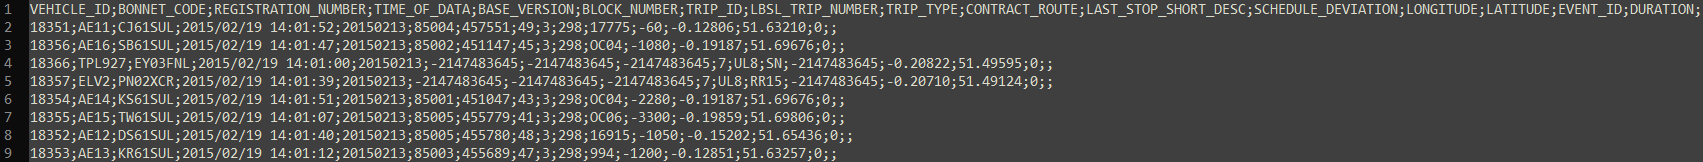
\includegraphics[width=1.7\textwidth]{Figures/ibusSampleRaw.png}}
	\caption{Sample Raw iBus Data}
\label{fig:rawDataSample}
\end{figure}

\begin{figure}[ht!]
	\makebox[\textwidth][c]{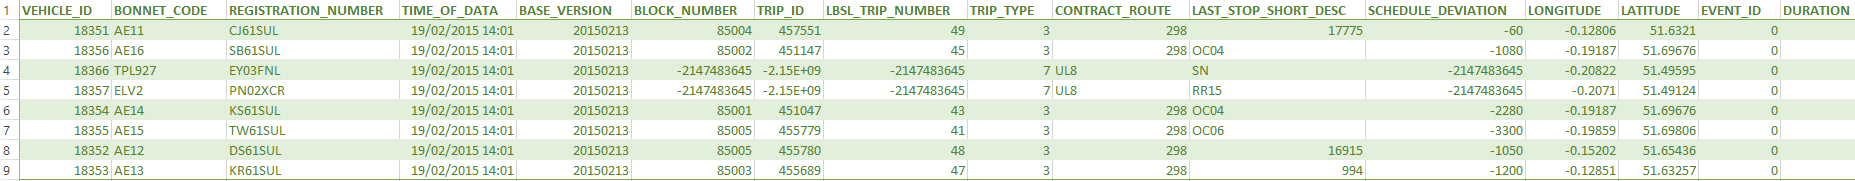
\includegraphics[width=1.7\textwidth]{Figures/ibusSampleFormatted.png}}
	\caption{Formatted Sample iBus Data}
\label{fig:formattedDataSample}
\end{figure}

\FloatBarrier
\section{Disruption Engine}
The disruption engine is implemented based on the design given in the previous chapter. The main implementation language used to the implementation is Scala. Scala is both functional and object oriented language \cite{odersky2008programming}. It is a type-safe Java Virtual Machine (JVM) language \cite{odersky2008programming}. This means that it is compatible with existing Java\footnote{\url{https://www.java.com/en/download/faq/whatis_java.xml}} code which allows for reuse of existing Java libraries. Scala was first introduced back in 2003, however, it has been only in the past few years that it had gained more popularity. In addition Scala enables the programmer to write more concise and clear code than one will can achieve in Java. The decision of using Scala has also been influenced by the fact that I have good knowledge of the object oriented programming paradigm as well as experience in Java. This allowed me to quickly pick up and learn Scala and put it into use.

The disruption engine needs to have an accurate internal representation of the bus network. TFL's bus network and any other bus network usually consists of bus routes. Each bus route often has multiple runs (directions - e.g. inbound and outbound). In turn, each run consists of a sequence of bus stops that the bus passes through. In addition to these typical bus network components, for our implementation we also have the notion of a section. By this we mean a pair of consecutive bus stops along a given run of a given route. In figure 5.1 below we can see an example for route 15 outbound where we have depicted two section X (between Leman Street and Tower Of London Stops) and Y (from Tower Of London to Great Tower Street). This means that if we have $n$ stops on a given run then we have $n-1$ sections on the same run.

\begin{figure}[ht]
	\makebox[\textwidth][c]{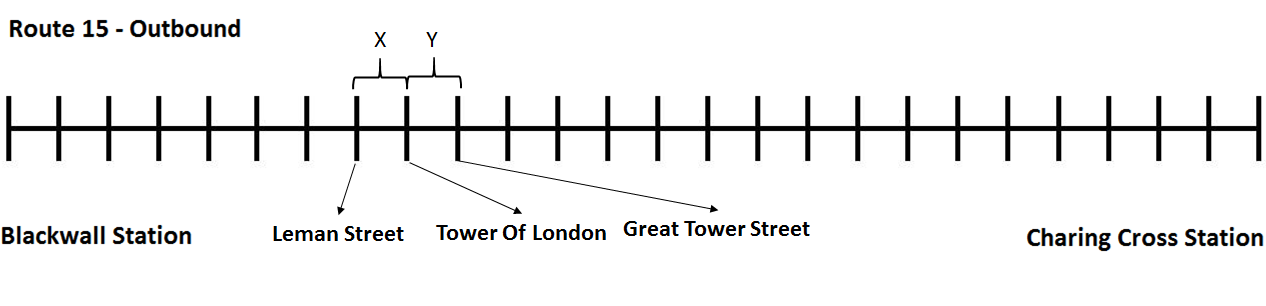
\includegraphics[width=1\textwidth]{Figures/sectionExample.png}}
	\caption{Example of a section}
	\label{fig:sectionExample}
\end{figure}

Our tool makes use of a PostgreSQL\footnote{\url{http://www.postgresql.org/about/}} database for storing all configuration parameters and also for storing the required information for the bus network representation. In figure~\ref{fig:dbModel} below, I have presented the relational model on which the database is based. The initial versions of the prototype used a CSV files as a means for storing the output. The decision to switch the flat file storage for a database is based on a number of things. The most important being is that using a database rather than CSV files we could keep historical data of the detected disruption for future analysis which is accomplished much easier using a proper database. Another advantage for the database approach is that it offers better concurrency support out of the box. Unlike the flat files which if manipulated concurrently could result in inconsistent state. Also having a database means that our disruption engine would require only details for establishing a connection to the respective database where it can read all other information that it requires. Otherwise it would require a number of other files and parameters to be defined which is not as easy to maintain as having one single database containing all of the configuration parameters as well as data for the bus network representation. For the above reasons I have decided to use PostgreSQL as it is advanced open source relation database management system. PostgreSQL has very good document and community support which is a big advantage for any technology. Another advantage for using PostgreSQL for our implementation is that it ensures reliability and data integrity \cite{lerner2007open}. Also it supports Listen\footnote{\url{http://www.postgresql.org/docs/9.1/static/sql-listen.html}} and Notify\footnote{\url{http://www.postgresql.org/docs/9.1/static/sql-notify.html}} functionality which could be used for real-time updating of the web application along with Server Sent Events (SSE) \cite{serverSentEvents}.

%However as other research has pointed out \cite{1251929} calculating travel time as measure for congestion is difficult task and it is very dependable on the environment and its conditions (e.g. weather, time of day, public demand etc.). For this reason and because of the data available this project would not try to measure disruptions by calculating travel time or bus speeds.TFL has provided us with example of the AVL data which among other things contains a the GPS coordinates of the bus at a given point in time and preprocessed deviation from the schedule value. For the rest of this chapter we assume this value is accurately calculated and that we would receive this value for each bus in the network at some regular interval. The provided data is discussed in further details in Chapter 5.
%For this project we monitor and measure the schedule deviation value as calculating the congestion is very challenging and still not very well understood in the case of arterial urban traffic.
%However from the literature \cite{1251929} we can see that it could be difficult to precisely define what we mean by congestion in a transport network. It seems that congestion could mean various things to different studies and people.
%What is the general approach I have taken
%WHAT ARE THE CHALLENGES AND HOW WERE THEY OVERCOMED
\begin{figure}
	\makebox[\textwidth][c]{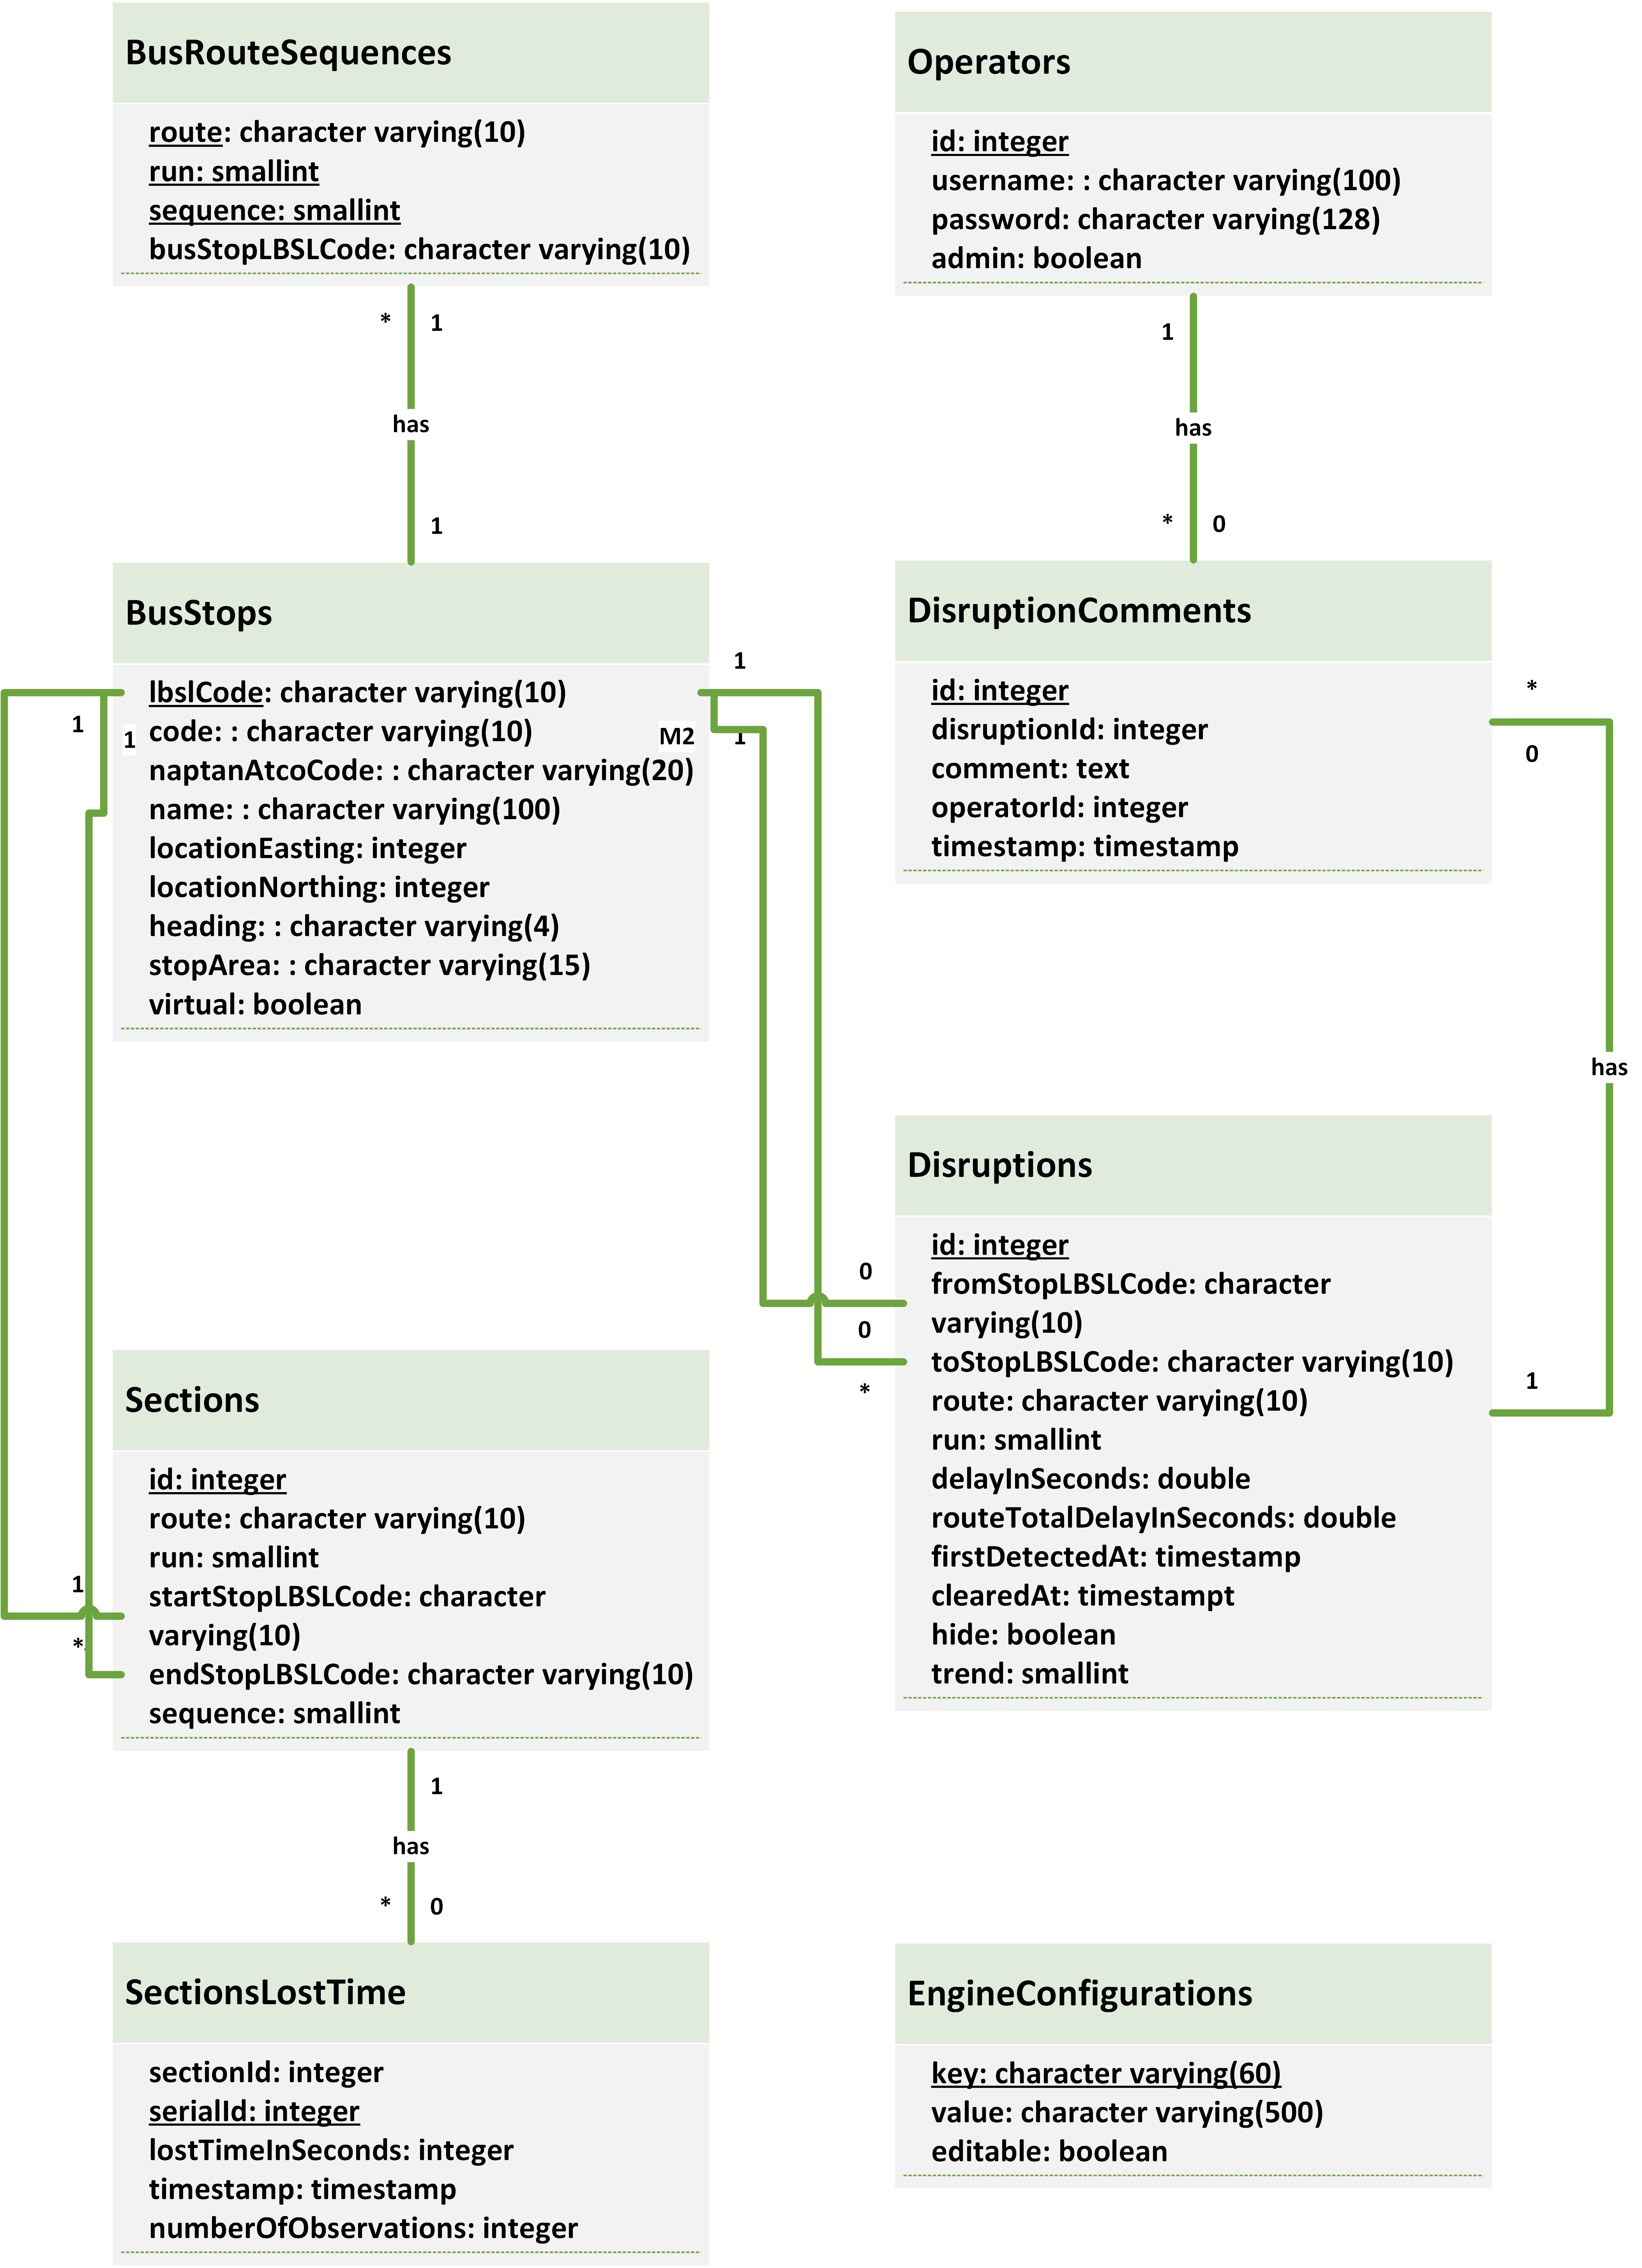
\includegraphics[width=1.2\textwidth]{Figures/DBModel.png}}
	\caption{Database Model Diagram}
\label{fig:dbModel}
\end{figure}

\FloatBarrier
\subsection{Bus Network representation}
In order for the engine to have full bus network representation, it requires information of the bus routes and the bus stops in the network. This information is freely available to anyone on TFL website \footnote{\url{http://www.tfl.gov.uk/info-for/open-data-users/our-feeds}}. It consists of two CSV files, one containing information on all bus routes and one for all bus stops in the network. The bus file contains a list of bus routes respectively has one or more runs which consists of sequence of bus stops. In our implementation we assume that this information is preloaded into the database. This preload consists of simply extracting the information from the CSV files obtained from TFL website into the respective tables (BusStops and BusRouteSequences). In addition to this we need to preload also the sections which will allows us to store individual section information. Currently sections are being generated manually however, this could be easily automated, but this is not in the scope of this project as it is most likely that TFL already have an internal database with this information in which case our tool will only require pointers to the respective tables. Then once the engine is started, it would read and load from the database all bus routes and respective sections. This results in the BusNetwork class storing a HashMap which maps a bus route name to the corresponding Route object. In turn, the Route class maintains a list of all runs for the respective route. BusStop information (apart from the bus stop LBSL code which we use as an id) is only loaded from the database on request. This whole process is part of the initialisation of the monitoring tool along with pre loading some other environment configuration parameters from the database. It happens only once throughout the execution of the tool and takes place just after the engine is started.

\subsection{Monitoring and processing new feeds}
Once the system is initialised, the tool will continuously monitor a specified directory (configurable from the database) for new feeds being written (pushed). Once new feed files are detected, they are picked up and processed by the engine. The processing consists of extracting the data of interest and calculating the time lost by buses on average for each section. Extracting the data means reading the CSV feed file line by line. Each line would be a data (observation) for a given bus thus we associate each observation with the route that is currently logged on. Once the observations are extracted, they are sorted by the time of the data field and any data that is older than a given predefined threshold (e.g. 120 minutes - this is configurable) is discarded. Once a given feed file is processed, it is moved to a predefine processed feed directory. This completes the feed file processing step. Feed processing is performed on batches of feeds (see the state machine diagram on figure A.5 in Appendix A). This means that once the engine detects new feed(s) in the directory it is currently monitoring, it will process all new feed files. 

\subsection{Bus network state update}
Once feed processing has finished, the system needs to update the bus network state. This consists of a number of steps. First we need to calculate the lost time per section. This process is done iteratively for every route in the network that has active buses (readings have been transmitted in some predefined interval of time e.g. 90 minutes). Each bus observation is then taken on a given route (see Figure~\ref{fig:example1}). At least two or more observations are required in order to calculate the time loss for a section. In the example below (figure~\ref{fig:example1}) we can take the first reading $x_1$ and the second reading $x_2$.
\begin{figure}[ht]
	\makebox[\textwidth][c]{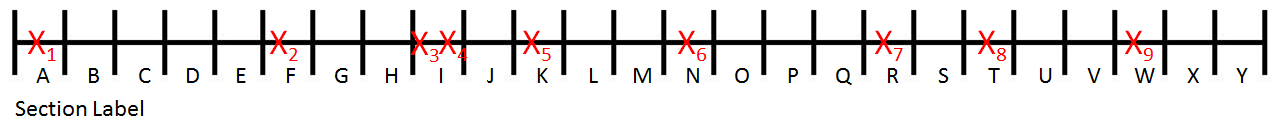
\includegraphics[width=1\textwidth]{Figures/implementationExample1.png}}
	\caption{Example of observations}
	\label{fig:example1}
\end{figure}
The difference in the schedule deviation between $x_2$ and $x_1$ is then calculated (see table figure~\ref{fig:example1Table}). 
\begin{figure}[ht]
	\makebox[\textwidth][c]{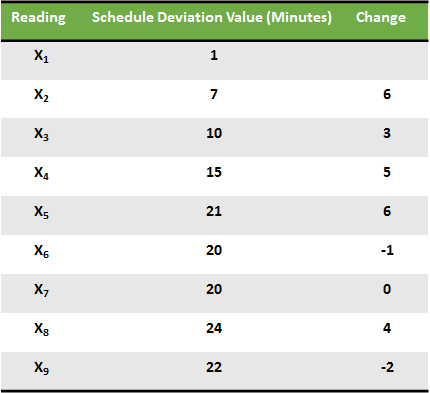
\includegraphics[width=0.8\textwidth]{Figures/implementationExample1Table.png}}
	\caption{Example schedule deviation calculations for the example in figure~\ref{fig:example1}}
	\label{fig:example1Table}
\end{figure}

Once we have calculated the schedule deviation change between two consecutive stops, we need to assign it to the respective sections. From our example we can see that reading $x_1$ has been sent somewhere from section $A$ and that $x_2$ from section $F$. This means that the bus have travelled through 6 sections ($A$ to $F$) and during that time it has lost $6$ minutes. The problem is that we do not know where exactly this delay has happened. It is possible that there was a delay just in one of the sections or it could have been distributed among all or few sections. For this reason what we do is to distribute this lost time evenly along all sections in-between the two readings. In our example this would mean that we would assign $1$ minute to each of sections $A$, $B$, $C$, $D$, $E$ and $F$. Then we take the next pair of observations, in this case $x_2$ and $x_3$ and do the same procedure. Every time we have new time loss value for a section, we add it to the existing lost time for the section and associate it with the newest observation time of the data. In this case that means section $F$ will have time loss value of $1+\frac{3}{4}$ and time-stamp equal to the time of data of observation $x_3$. If we however, take the case of reading $x_3$ and $x_4$ we know for sure that the delay has occurred in section $I$ thus we assign the $5$ minutes lost time only to section $I$. Repeating the above steps for each bus on a route will result in a list of values representing the delay (time lost) and the time (time of the data of the latter observation in the examples given above this means we take the time of the data of $x_2$ and $x_4$ respectively) when this has occurred.
 
Once we have a list of these values for each section of each bus route, we need to calculate the weighted moving average of this data. To do this we firstly need to sort this list of values for each section of a route run by the time of the observation in ascending order. Then we calculate the weighed moving average by assigning the oldest data weight of $1$ and the newest data weight of $n$ ($n$ is the number of data entries of a section). Calculating the weighted moving average instead of a simple average, we put more weight on the newer data and also help dampen the effect of a single irregularity (e.g. a bus has experienced a technical fault).

Doing the above steps, we obtain a value representing the WMA time loss (delay) for each section (see figure~\ref{fig:example3}). The next step then is to examine each route run and its sections in particular and check if any of them are disrupted. To accomplish this we firstly check if the total cumulative lost time of the sections of the respective run, is greater than or equal to some predefine minimal threshold (this is configurable). In case this does not hold (e.g it is below the minimal threshold) the algorithm will move onto the next run and will consider this one as clear (without any problematic sections). Any negative values (e.g where buses have gained time) are treated as $0$, as we are only interested if there are any problematic sections along the route run.

However if for example we assume that the minimal threshold is $20$ minutes and take the example from figure~\ref{fig:example3} we can clearly see that the cumulative lost time is greater than or equal $20$. In such cases we need to look more closely at this route run and try to identify the sections which are causing the most delay. We do this by searching for a number of consecutive sections which have their sum of the delay time greater or equal to some predefined threshold (e.g. 20 minutes). However, small delays (e.g of $1$-$2$ minutes) are treated as $0$ as there are always some slight variations and we are only interested in major disruptions which are beyond the control of individual bus operator companies. If we take the example presented in figure~\ref{fig:example3}, we can see that there seems to be some significant problem between sections $L$ and $O$. The sum of the delay is $7+14+12+5 = 36$ minutes which is greater than our example threshold of $20$ minutes. This results in the engine detecting and outputting a disruption between those sections.

\begin{figure}[ht]
	\makebox[\textwidth][c]{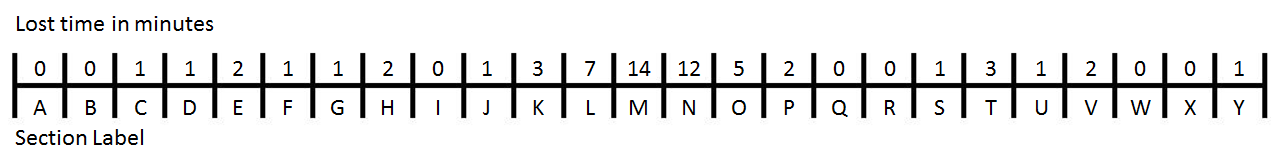
\includegraphics[width=1\textwidth]{Figures/implementationExample3.png}}
	\caption{Example of a disruption}
	\label{fig:example3}
\end{figure}

However, we have to limit the number of consecutive section we look at a single time as for example we consider the below case (see Figure~\ref{fig:example2}). We can have a long route run with very small loss of time per section (as in the example below, of the order of $1$ to $3$ minutes) but overall they might add up to $20$ or more minutes in particular if the route run is long (e.g has 30 or more stops). This however, does not represent a single problematic hotspot and is responsibility of the bus operators to manage such cases and not CentreComm. For this reason our algorithm would mark the start of a disruption as the first section it encounters with a greater WMA delay value and it would continue expanding this specific disruption until it finds/reaches a section with value less than the minimal threshold for section time loss value or the end of the run. Then it checks if the total delay for the detected sections is greater than or equal to the minimal disruption threshold. If true, it outputs it as a disruption affecting those sections. This is done for the rest of the route run even if some disruptions are already detected at the beginning of the run of a particular route.

\begin{figure}[ht]
	\makebox[\textwidth][c]{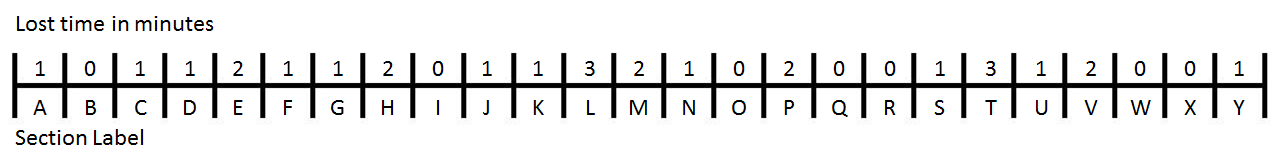
\includegraphics[width=1\textwidth]{Figures/implementationExample2.png}}
	\caption{Example of no disruption}
	\label{fig:example2}
\end{figure}

Every detected disruption or one such that it has changes in its state is updated and written to the database. This allows for the user interface to update itself with the latest information. The engine also writes a snapshot of the sections state of every route run in the network which has active disruptions. We only write data for the sections which belong to runs with disruption due to performance considerations. For example if we take the London bus network which has $680$ routes most of which have $2$ runs (outbound and inbound) and each run on average has $30$ stops, it means we have more than $40000$ sections. Updating them each time would take significant computational time (e.g. couple of seconds depending on the machine and the location of the database) and also would be waste of space. For this reason our implementation only updates sections which belong to disrupted runs as this information is utilised for displaying detailed graphs in the user interface.

%This is also the scenario where diversions become problematic.
%Once we have calculated the weight moving average time loss per section, we need to check if there are any sections that are of interested and need to be displayed (e.g. are there any disruptions).
%Here one problem arises as we need to take into account diversions. More details on this problem can be found in the section below. If we just ignore disruption we need to find if there is a number of consecutive sections which have their sum of the loss of time greater or equal to some predefined threshold (e.g. 20 minutes). For example in the example (see Figure 2) below we can see that section 5, 6 and 7 add up to 24 minutes of delay and thus we output that there is a disruption between stops E and H. 
%The next step is to calculate the weighted moving average of this data. We do this by taking the list for each section and sorting it by the time of the observation (e.g in the above example section 1, 2 and 3 would have time of the data equal to the x\textsubscript{2} observation).  
%Lets assume this difference is 3 and we can see that reading x\textsubscript{1} has been send from the first section of the route and reading x\textsubscript{2} from the the third section of the route. This means that the bus has lost 3 minutes between these two points on the route. However we cannot know for sure which section or sections have caused this loss and we can only distribute this loss equally between the three section. This means that each of section 1, 2 and 3 would be assigned 1 minute of loss. If we take however the case of reading x\textsubscript{3} and x\textsubscript{4} we can be very confident that the loss has occurred in section 5.

\FloatBarrier
\section{Graphical User Interface}
The engine implementation described above addresses only half of our requirements. In order to fully meet the project goals we need to be able to visualise the detected disruption in the network. For this reason we need to produce some kind of user interface which to be able to meet the requirements for visualisation of the detected bus delays. As described in section 4.5 of this report, we have decided to have individual application for the back-end disruption engine and the user interface. For the implementation of the user interface we have chosen to create a web application using Ruby\footnote{\url{https://www.ruby-lang.org/en/}} as the programming language running on Rails\footnote{\url{http://rubyonrails.org/}} framework.

The Rails framework is full stack open source web framework implemented in Ruby which allows for quick development and deployment \cite{guide2006agile}. It is relatively easy to use and maintain and it supports a wide range of software engineering paradigms and patterns. The main ones being Model View Controller (MVC), Don't Repeat Yourself (DRY), Convention Over Configuration (CoC) and the Active Record pattern \cite{fowler2003patterns}. Ruby is object-oriented scripting language which is famous for its conciseness. It enables the programmer to express his intentions quickly in very few lines code and it is also easy to read this code later (in future). Another advantage that Rails framework provide is the automatic code generators which provide code skeletons which save effort and time. Rails also allows for agile software development as this is in its roots \cite{guide2006agile}. It is also important to note that Rails has a strong support community and documentations as well as expansive list of add-ons and third-party libraries.

Other languages and framework have also been considered to be used instead of Ruby and Rails for this project. However, the chosen ones provide us with technologies which are to be used for quick prototyping and agile development which our project is following. In addition to the above this was also an opportunity for me to learn a new language and framework which I have not used before.

I have also made use of Foundation \footnote{\url{http://foundation.zurb.com/}} Cascading Style Sheets\footnote{\url{http://www.w3.org/Style/CSS/Overview.en.html}} (CSS) front-end framework. This framework has enabled quick prototyping as it has a rich library of predefined components. However, its main advantage over some other similar frameworks is its notion of grid which allows for quick and easy implementation of responsive websites. Making the web application with responsive design allows us to reach more platforms and client systems with a single application. This allows us with little additional implementation effort and time to achieve results which look good on both large screens (desktop computers, laptops etc.) as well as on small screen and mobile devices (e.g. smart phones, tablets etc.). This framework also has the advantages of good support in terms of documentation and add-ons and it is lightweight.

%Sample of what the system user interface looks like can be seen in appendix A [REFERENCE TO APPENDIX]. 
%For this reason I have decided to implement the visualisation part of the system as a separate web application. The advantages of this approach are that this provides universal access to the information. We only need to deploy this application once and it can be accessed from multiple clients running different operating systems and even devices. I have decided to use Ruby running on Rails framework. The reason for this is its recent popularity and wide support in terms of third party libraries and community information and guides.
%The Rails framework [REFERENCE] is full stack open source web framework implemented in Ruby.

The ruby on rails web application is implemented following the MVC pattern. MVC allows the programmer to structure their application code better with clear separation of concerns. In our case it consists of few simple models representing the corresponding database tables, controllers and a number of views. The models are implemented as Active Records\footnote{\url{http://guides.rubyonrails.org/active_record_basics.html}} which provide interfaces to the respective database tables. They provide create, read, update and delete (CRUD) functionalities. The controllers are responsible for processing the client request by parsing and checking for any parameters, credentials where necessary and responding with the requested information. The responses are, in most cases rendered views containing the requested information.

The user interface can be seen in figures~\ref{fig:ui1} to~\ref{fig:ui10}. It consists of three main views which are the disruption view (figure~\ref{fig:ui1}), the history view (figure~\ref{fig:ui3}) and the settings view (figure~\ref{fig:ui8}). The main view is the disruption one which is responsible for visualising the disruptions in the network at any point in time. The list is displayed in tabular form (figures~\ref{fig:ui1}). This provides instant awareness of what the network state is to the CentreComm operators. Disruptions are prioritised by their severity and are colour coded.

The application also has a basic authentication in place which enables to distinguish between the three type of users as described in section 4.1. Guest users do not have to authenticate, but they have limited access meaning they have read-only view of the system. The system also allows users to login in (figure~\ref{fig:ui4}) and depending on their status they could either be operators or administrator users. The administrator users have full access to the functionalities which includes view of the settings and the ability to change them, this is not possible if you are guest or operator user. Logged in users are allowed to hide/show (the result is that guest users would not see hidden disruptions) disruptions (figure~\ref{fig:ui7}) and also to add comments (figure~\ref{fig:ui10}). All users including guest are enabled to request further information for a given disruption which includes a graph of the lost time on the disrupted route see figure~\ref{fig:ui2}. This graph is a combo chart\footnote{\url{https://developers.google.com/chart/interactive/docs/gallery/combochart}} (combination of line and bar chart) and is created using Google Charts\footnote{\url{https://developers.google.com/chart/}}. The bars of the graph denote the WMA delay per section while the line depict the cumulative lost time along the route (this treats all negative values as $0$). The Google Charts API\footnote{API - Application Program Interface} allows us to make the graph interactive such that on hoover we can display more detailed information for the selected section which allows us to create a clear and organised layout with all the information available. This graph is very useful as it provides the CentreComm operator or other users with a detailed view of what is the state of the given route. The real-time disruption list and the history table are by default sorted by severity of the section delay and the total delay. However users are enable to sort by any other column. This is achieved using Ajax \footnote{Short for asynchronous JavaScript and XML} in order to minimise network load by only reloading the changed part of the web page (we do not need to reload the navigation menus, footers etc.). I have also added a data filter for the history view. The history view has not been part of the initial requirements or aims of the project, but it has been identified as great benefit tool like ours can offer. Because of this it has been added during the later stages of the project just as a proof of concept.

%The disruptions at any point in time are visualised in tabular form. Disruptions are prioritised by their severity and are color coded. Further details for disruption are displayed on request of the user. This includes a graph representation of the delay observed on each section along the disrupted route. On this graph the cumulative delay for this route is also visible. When hovered the graph displays details for this section including the start and end stop of it and the number of observations.

One important aspect of the user interface is how to update the disruption list in real time whenever there are changes. This is achieved by implementing Ajax short polling \cite{bozdag2007comparison}. This means that we use asynchronous JavaScript on the client side to make request to the server at predefined intervals. Alternative methods for implementing the updating of the list include WebSockets\footnote{\url{https://tools.ietf.org/html/rfc6455}}, Ajax Long Polling \cite{bozdag2007comparison}, Server Sent Events (SSE)\cite{serverSentEvents}. The main advantage of using Ajax short polling over WebSockets and SSE are that Ajax Short Polling is supported by all major web browsers natively unlike SSE which lacks Internet Explorer support. Also it does not require the set-up of any additional tools or infrastructure unlike WebSockets. The drawback of using Ajax polling is that in order to achieve near real time update, the clients will need to make frequent request to the server which wastes network bandwidth and server resources. SSE is the best approach in this scenario as it establishes a persistent long-term connection on which the server is able to push new data once it becomes available to all connected clients. However SSE is relatively new standard and it is has been standardized only as part of HTML5\footnote{\url{http://www.w3.org/TR/html5/}}. As mentioned above Internet Explorer does not support SSE and this is a major drawback in our scenario as this is one of the main web browsers CentreComm staff use. In addition to this, SSE require the use of a concurrency enabled server. WebSockets provide a persistent two-way connection between the client and the server however, in our case we are mainly interested in pushing new data from the server to the client. There is very little information the clients need to send to the server and thus we have excluded this approach as viable one.

\section{Problems}
During the implementation of the project a number of obstacles and problems have arisen. In this section we discuss the major ones. All that are not mentioned below are assumed to be solved by our implementation and not of enough significance for the reader.

The main challenge during the implementation has been how to assign the lost time between two consecutive observations to the respective sections that the bus has travelled through. This is because the data we work with is sparse (currently every 5 minutes) which means that during the time between those two observations the bus could have passed a number of sections and bus stops and we will only know the last bust stop it has attended. To solve this problem our the disruption engine keeps an ordered list of observations for each unique vehicle which is active on a given route. To assign the delays accordingly, the engine takes two observations at a time and does a number of steps. The first step is to check if the observations that have been made along the same run (e.g. both readings come from the bus when it was travelling outbound along the respective route). To do this we need check if the last stop from the earlier observation and the last stop from the latter reading are both from the same run and the earlier is preceding the latter last stop.

One problem that was encountered is that there is no explicit information in the data that has been provided if a bus is on diversion. Diversions vary greatly in terms of length (few or many stops) and duration (e.g. it can last half an hour or few weeks/months) of the implemented diversion. What happens in such cases is that the bus would still transmit its position, but the central iBus server would not be able to calculate the schedule deviation. This results in readings in the feed file which have abnormal values for the schedule deviation and other fields. These abnormal values however, are always the same and are equal to the negative integer $-2147483645$. However, this does not happen only when the bus is on diversion, it can also happen if there is problem with the GPS (e.g. weak signal due to high buildings) of the respective bus or if the bus is not logged on properly in the iBus AVL system. This means that we are unable to know for sure what such readings mean. For these reasons when such readings are observed by the engine they would simply be ignored. The implications of this are that our implementation loses some accuracy and it may produce delayed alerts. If we consider the example shown on figure~\ref{fig:diversion} where buses on this route are on diversion from section $F$ to section $P$, what will happen is that we will get correct data before and after the diversion which would be processed. However, during the diversion, the data we will get from the buses currently travelling on this diverted path will have meaningless values and thus the disruption engine will ignore it. This means that if buses experience delay during the diversion this would only be picked up by the system once they return on the normal route. However, the delay that the system will observe would be distributed along the whole diversion (as described above in section 5.1). This means that in case we have long diversion some significant delay might not be picked up by the system. This can also happen if there is problem during part of the diversion, but during the rest of the diverted route the buses actually manage to get back on schedule.

\begin{figure}[ht]
	\makebox[\textwidth][c]{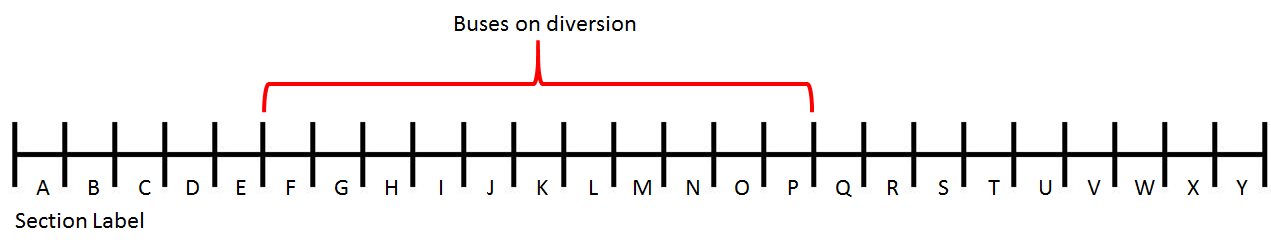
\includegraphics[width=1\textwidth]{Figures/diversion.png}}
	\caption{Example of diversion}
	\label{fig:diversion}
\end{figure}

Another problem with the available data is that we do lose some accuracy (some readings are ignored) when the bus turns at the end of a run. We cannot simply assume that every bus would travel along a route from start to end and turn as there are occasions when buses are curtailed\footnote{To cut short.} along the route. This can happen for a number of reasons including service regulation, heavy congestion/disruption along some sections of a route, bus driver exceeding the allowed by law work hours and more.

Our system relies on monitoring for changes in the schedule deviation value as indicator for the delays in the network. However, there are some scenarios where the engine can detect delays where in fact there are no real-life disruptions taking place. To understand why this can happen, consider the case when a bus is initially ahead of schedule. This can result in the bus driver or operator company to deliberately force this service to lose time in order to be right on time. This is especially a problem for low frequency buses as they run according to fixed schedule and not based on headways. Thus we can claim that our implementation provides an upper bound of the disruption delays in the bus network.

Another problem of the approach taken is that because the system relies on monitoring the schedule deviation value and it does not treat differently calculations where during the first observation the bus is ahead or schedule and when it is already behind. This means that it is possible that the bus driver is losing time on purpose for service regulations. Thus we can assume that our tool provides an upper bound of the disruption.

Some other problems with the implementation include inconsistencies in the bus route sequence data. This however, is affecting small number of routes and does not prevent our system from delivering a proof of concept. This issues have been discussed with members of the TSG and have been considered irrelevant for the purpose of this project. However, it has been agreed that they would need to be addressed in case this is tool is put into production. 

%When such readings are observed by the engine they would simply be ignored. This is problematic and our system only ignores it in the current prototype as failure in computing the schedule deviation could also be caused by the bus not being properly logged into the iBus system (e.g. bus taking a break at end of route). This means that we lose some accuracy especially for longer diversions as any lost time would be distributed along the sections which have not been observed (where the bus has been on diversion). This however could also be the case if a bus skips or fails to send data. Again this could be because of number of reasons (e.g. weak signal due to high buildings etc.).

%The important factors to consider are the weights and the period/window size to use. We could also apply exponential smoothing on top of the WMA.
%Problems:
%The bus could have started the journey ahead of schedule and thus to intentionally be losing time.
%The buses could curtail anywhere on a route without notification
%The buses could be diverted (this could be short term or long term) it can also be for few stops or it could be a longer diversion.

%PROBLEM - some buses might skip transmitting data even if they are properly logged on
%Data available, data frequency, no knowledge when buses do curtail, not taking into account bus dwell time, bus drivers who are running ahead of schedule could be driving slower on purpose and thus. Tool gives an upper bound of the of the WMA lost time per section. 
